\documentclass[%
%preprint,
 reprint,
superscriptaddress,
%groupedaddress,
%unsortedaddress,
%runinaddress,
%frontmatterverbose,
showpacs,preprintnumbers,
%nofootinbib,
%nobibnotes,
%bibnotes,
 amsmath,amssymb,
 aps,
 prl,
%pra,
%prb,
%rmp,
%prstab,
%prstper,
%floatfix,
]{revtex4-1}
\usepackage{natbib}
\usepackage{graphicx}% Include figure files
\usepackage[caption=false]{subfig}

\usepackage{siunitx}
\usepackage{dcolumn}% Align table columns on decimal point
\usepackage{bm}% bold math
\usepackage{hyperref}% add hypertext capabilities
\usepackage[mathlines]{lineno}% Enable numbering of text and display math
\usepackage{mathtools}
\usepackage[percent]{overpic}
% \linenumbers\relax % Commence numbering lines %WARNING: not work with subfig!

%\usepackage[showframe,%Uncomment any one of the following lines to test
%%scale=0.7, marginratio={1:1, 2:3}, ignoreall,% default settings
%%text={7in,10in},centering,
%%margin=1.5in,
%%total={6.5in,8.75in}, top=1.2in, left=0.9in, includefoot,
%%height=10in,a5paper,hmargin={3cm,0.8in},
%]{geometry}
\DeclareSIUnit\basepair{bp}

\newcommand{\gwlc}[2][\Omega_0; L_0]{G_\text{\tiny WLC}(#2|#1)}
\newcommand{\ghat}[2][\Omega_0; L_0]{\hat{G}_\text{\tiny WLC}(#2|#1)}
\newcommand{\greens}[2][\Omega_0; L]{G(#2|#1)}
\newcommand{\pathd}[1]{\mathcal{D}\left[#1\right]}
\newcommand{\energy}{\mathcal{E}}
\newcommand{\wigD}{\mathcal{D}}
\newcommand{\RR}{\left\langle{}R^2\right\rangle{}}
\newcommand{\meanli}{\left\langle{}L_i\right\rangle}

\begin{document}
%\preprint{APS/123-QED}
\title{Heterogeneity in Nucleosome Spacing Governs Chromatin Elasticity}% Force line breaks with \\
\thanks{A footnote to the article title}%

\author{Bruno Beltran}
\thanks{These authors contributed equally to this work.}%
\affiliation{%
    Biophysics Program, Stanford University, Stanford, California 94305, USA
}%
\author{Deepti Kannan}%
\thanks{These authors contributed equally to this work.}%
\author{Quinn MacPherson}%
\affiliation{%
    Department of Physics, Stanford University, Stanford, California 94305, USA
}%
\author{Andrew J. Spakowitz}%
\email{ajspakow@stanford.edu}%
% \homepage{http://web.stanford.edu/~ajspakow/}%
\affiliation{%
    Chemical Engineering Department, Stanford University, Stanford, California 94305, USA
}%
\affiliation{%
    Department of Materials Science and Engineering, Stanford University Stanford, California 94305, USA
}%
\affiliation{%
    Department of Applied Physics, Stanford University, Stanford, CA 94305
}%
\date{\today}% It is always \today, today,
             %  but any date may be explicitly specified

\begin{abstract}
\textit{In vivo}, the myriad of proteins that bind DNA introduce heterogeneously-spaced
    kinks into an otherwise semiflexible DNA double helix.
% % theta given 0 unwrap...
% Most notably, in a nucleosome, DNA winds around the histone octamer to form an
%     effective \ang{62.7} bend, a conformation that is thermally inaccessible to
%     bare DNA\@.
We present an analytical model for the effects of these rigid kinks on the
    physical organization of chromosomal DNA\@.
For periodic kinks, the elasticity of chromatin chains is extremely sensitive to
    nucleosome repeat length.
In contrast, we show that heterogeneity in nucleosome spacing eliminates this
    sensitivity, allowing us to robustly predict the Kuhn length of chromatin in
    various cell types.
In addition, we find that by merely rearranging the positions of intervening
    nucleosomes, it is possible to change the probability that two genomic
    loci loop together by up to 6 orders of magnitude.
Finally, we show that on time scales longer than nucleosome turnover, chromatin
    is well described by an effective WLC with the persistence length we
    calculate.
Our results are broadly applicable to any semiflexible polymer with aperiodic
    defects, and the their implications for the flexibility and cyclizability of
    block copolymers are discussed.
% We discuss the effects of nucleosome repositioning on the structure and
%     topology of chromatin loops.
\end{abstract}

% PACS, the Physics and Astronomy Classification Scheme.
\pacs{05.20.--y, 05.40.Fb, 36.20.Ey, 87.10.Ca, 87.14.gk, 87.15--v, 87.16.Sr}
%Use showkeys class option if keyword display desired
%\keywords{chromatin \| nucleosome \| kinked WLC}
\maketitle


% \section{\label{sec:intro}Introduction}
%TODO bad hbox when attempting line break of the following sentence
In the cell, DNA and its associated proteins---collectively, chromatin---are
    carefully organized both spatially and temporally.
This organization is known to play a role in a myriad of biological processes,
    from controlling gene expression~\cite{hubner2013} to facilitating DNA
    damage repair~\cite{hauer2017,stadler2017}, and has motivated a large body
    of work on the statistical mechanics of the chromatin fiber.

The fundamental repeating unit of Eukaryotic chromatin organization is the
    nucleosome, which is formed by 147 basepairs of DNA wrapped around a histone
    octamer~\cite{cutter2015a}.
Linker DNA connecting adjacent nucleosomes ranges from $<$\SI{10}{\basepair} on
    average in fission yeast~\cite{givens2012} to {$\approx$\SI{50}{\basepair}} in human
    cells~\cite{schones2008}.
Nucleosomes, along with their intervening linkers, are collectively referred to
    as the ``beads on a string'' model of the chromatin fiber.

While numerous simulation studies have highlighted the importance of linker
    lengths on the structure of chromatin~\cite{bascom2017a,
    collepardo-guevara2014, bascom2018, grigoryev2016, kepper2008, koslover2010,
    langowski2007, muller2014, schiessel2001, scipioni2010, wedemann2002,
    woodcock1993%
    %these are "meh" norouzi2015, stolz2010,
    }, no analytical framework exists to unify these disparate results and
    provide general guidance for coarse-grained models of chromatin.
As a result, most simply treat chromatin as an effective
    wormlike chain (WLC), where the persistence length $l_p$ is chosen to either
    arbitrarily match that of bare DNA~\cite{benedetti2017, macpherson2018,
    nuebler2018} or to fit the quantity being
    measured~\cite{sanborn2015,pierro2017}.

Our lab previously published an analytical treatment of the beads on a string
    model (with WLC linkers) for the special case of constant linker
    lengths~\cite{koslover2013a}.
However, nucleosomes in the cell are almost never perfectly spaced.
The occupancy profiles of even the most well-positioned nucleosomes---such as
    those near transcription start sites---are well described by a model where
    nucleosomes instead bind uniformly along the DNA~\cite{kornberg1988,%
    %extra
    chevereau2009, chereji2011, beshnova2014, chou2007, kornberg1981,
    mavrich2008, mobius2010, mobius2013, teif2010, tesoro2016%
    %indirect locke2010,
    %foundational math mcghee1974, vanderlick1986
    %belongs in extra but i'm morally opposed to giving credit: schopflin2013
    }, and
    are merely excluded from certain areas~\cite{ozonov2013}.
% These models are referred to as the ``lattice gas'' picture of nucleosome
%     binding, after the Tonks gas they generalize.


%BRUNO: consider including the following if there's space
%The main disagreement between these lattice-gas models and experimental data
    % was due to the experimental data being more ``smooth'' than the
    % model~\cite{beshnova2014}.
%This inspired many additions to the model, most
    % notably, introduction of non-nucleosome non-specific DNA binding
    % proteins and partial nucleosome unwrapping~\cite{beshnova2014}.
% However, recent single-cell MNAse-seq data~\cite{lai2018} do not show this
    % discrepancy\footnote{Compare the red and green curves in Figure 2a and 2c
    % of \citep{lai2018} to see how pooling multiple cells can cause the effects
    % that \citep{beshnova2014} attempt to prevent by adding unwrapping to their
    % model.}, suggesting that the most naive lattice gas
    % model with uniform binding and no unwrapping can likely explain nucleosome
    % positioning in human cells.

In this paper, we extend our analytical theory to incorporate arbitrarily spaced
    kinks, and use it to investigate the effects of realistic nucleosome spacing
    on chromatin structure.

We first show how the zero-temperature limit---where the chain simply consists
    of rigid rods held together by nucleosomes---provides a simple intuition for
    the effects of kinks in a WLC.\@
We use this intuition to show how, for heterogenous linker lengths,
    chromatin's structure exhibits a kind of universality.
Namely, the structure is independent of the particular distribution of the
    linker lengths.
This result allows us to calculate looping probabilities and the Kuhn length
    of chromatin as a function of the average linker length without specifying a
    detailed model of nucleosome binding.
By comparing our results to a simple wormlike chain, we show that over time
    scales longer than nucleosome turnover, an effective WLC is sufficient to
    describe the average structure of the chain.
However, at shorter time scales, when individual nucleosome positions are
    essentially fixed, we show that the formation of large-scale functional
    chromatin loops can be precisely modulated by local changes to nucleosome
    positions.

% Our simple model fills an important gap by providing physical intuition for how
%     nucleosome positioning guides chromatin organization.

\section{\label{sec:model}Model}
First, we make rigorous our ``beads on a string'' model of chromatin.
We treat each DNA linker as a WLC and nucleosomes as the points where these
    WLC's are connected.
At each nucleosome, we impose the constraint that the incoming and outgoing
    linker DNA strands have a fixed relative orientation. This relative
    orientation $\Omega_\text{kink}  = {(\Omega^{(i)}_\text{entry})}^{-1}
    \Omega^{(i)}_\text{exit}$ between the $i$th and $(i+1)$th linkers is
    determined by the nucleosome structure, as shown in
    Figure~\ref{fig:nuc-geo}.

We represent this sequence of WLC's as a space curve $\vec{R}(s)$, $s\in[0,L]$. 
    The chain's orientation at each point along this curve, $\Omega(s)$ is
    represented by the orthonormal triad
    $\vec{t_i}$, where $\vec{t_3} \coloneqq \partial_s \vec{R}(s)$.
We track the bend and twist of our polymer via the Euler vector $\vec{\omega_i}$
%why is there an Omega(s) here? I thought Omega represented the orientation
%triad
    defined by ${\partial_s \vec{t_i}(s) = \vec{\omega_i}(s) \times
    \vec{t_i}(s)}$.

We begin by computing the Green's function of the first linker, which represents
the probability that the polymer of length $L_1$, which begins at
the origin with fixed initial orientation $\Omega_0$, will end at position
$\vec{R}$ with fixed end orientation $\Omega$.
For a twistable WLC with no kinks, the Green's function is given by
\begin{equation}\label{eq:path}
    \gwlc[\Omega_0;L_1]{\vec{R}, \Omega} =\! \int_{\Omega_0}^{\Omega} \!\! \pathd{\Omega(s)}
              e^{-\beta \mathcal{E}}\delta(\vec{R} - \!\int_{0}^{L_1} \!\!\vec{t_3} ds),
    % overflows: yes, but it's an orientational integral, not over position.
              % How's the above? ^^
    % \greens{\vec{R}, \Omega} = \int_{\Omega(s=0)}^{\Omega(s=L)} \pathd{\Omega(s)}
    %           \exp{[-\beta \mathcal{E}]}
    %           \delta\left(\vec{R} - \int_{s=0}^L \vec{t_3} ds\right)
\end{equation}
    where the energy
\begin{equation}\label{eq:energy}
    \beta\energy = \frac{l_p}{2}\int_{0}^{L_1} ds
    (\omega_1^2 + \omega_2 ^2) + \frac{l_t}{2}\int_{0}^{L_1} ds
    {\left(\omega_3 - \tau\right)}^2
\end{equation}
%TODO get citations for DNA structure things
    is quadratic in bend and in twist. {$\tau \approx \SI{10.5}{\basepair}$}
    per turn is the equilibrium twist density of the DNA double helix, and {$l_p
    \approx \SI{50}{\nano\metre}$}, {$l_t \approx \SI{100}{\nano\metre}$} are
    the bend and twist persistence lengths of DNA, respectively.

This equation can be solved analytically in Fourier space
    ($\vec{R} \rightarrow \vec{k}$) by expanding in Wigner
    D-functions~\cite{spakowitz2006}, analogs of spherical harmonics for
    $SO(3)$.
%TODO equation overflows if a period is added
\begin{equation}\label{eq:expansion}
    \ghat{\vec{k}, \Omega} = \sum_{l m j}\sum_{l_0 m_0 j_0} \!\! g_{l_0 m_0 j_0}^{lmj}
        \wigD_l^{mj}(\Omega)\wigD_{l_0}^{m_0 j_0 *}(\Omega_0)
\end{equation}
In order to account for the kink introduced by the nucleosome, we rotate
    the final orientation of the linker DNA ${\Omega = \Omega_\text{entry}}$ to
    $\Omega_\text{exit}$ by replacing
%DEEPTI: why the paranthetical 1? seems unnecessary
%BRUNO: to match first paragraph of intro
%DEEPTI: my derivation has this as Omega_kink inverse?
%TODO check that the Omega_kink convention matches supplement
    $g_{l_0 m_0 j_0}^{lmj}$ in Eq.~\ref{eq:expansion} with
    \begin{equation}\label{eq:coeffs}
        B_{l_{0}m_{0}j_{0}}^{lmj} = %\sqrt{8\pi/(2l+1)}
        \sqrt{\frac{8\pi}{2l+1}}
        \mathcal{D}_{l}^{jj_{0}}
        \left(\Omega_{kink}\right)g_{l_{0}m_{0}j_{0}}^{lmj}\left(L\right).
    \end{equation}
    The resulting greens function combines the effects of a linker and a
    nucleosome.
The coefficients $B_{l_0 m_0 j_0}^{lmj}(\Omega_\text{kink}, L)$ were first
    computed in~\cite{zhou2003}, and an alternative derivation can be found in
    the supplement.

\begin{figure}[t]
    \centering
    \subfloat[]{\label{fig:entry-exit}
        \begin{overpic}[width=100pt]{./figures/fig-1a-nucleosome-geometry.png}
            \put(16,-3){\large$\displaystyle\theta$}
            \put(10,59){\large$\displaystyle\Omega_\text{entry}$}
            \put(62,17.5){\large$\displaystyle\Omega_\text{exit}$}
        \end{overpic}%
    }\hfill{}
    \subfloat[]{\label{fig:linker-effect}
        \begin{overpic}[width=130pt]{./figures/fig-1b-helicity-effect.png}
            \put(17,11){\parbox{1.5cm}{\centering DNA Helicity}}
            \put(-2,47){\large$\displaystyle\phi$}
            \put(-6,63){$\displaystyle\SI{33}{\basepair}$}
            \put(11,77){$\displaystyle-\SI{2}{\basepair}$}
            \put(40,81){$\displaystyle\SI{35}{\basepair}$}
            \put(61,72){$\displaystyle+\SI{2}{\basepair}$}
            \put(76,46.5){$\displaystyle\SI{37}{\basepair}$}
        \end{overpic}
    }%
    \caption{\protect\subref{fig:entry-exit} The structure of a
        human nucleosome~\cite{wakamori2015} with straight linkers extrapolated
        based on the entry ($\Omega_\text{entry}$) and exit ($\Omega_\text{exit}$)
        orientations of the bound DNA\@.
    The amount of DNA wrapping the nucleosome dictates the spherical angle
        $\theta$.
    \protect\subref{fig:linker-effect} Two adjacent nucleosomes at zero
        temperature.
    The DNA double helix has an intrinsic twist density
        $\tau=\SI{10.5}{\basepair}$.
    If we anchor the location of one nucleosome, the
        binding orientation of the next histone octamer must change so that it
        aligns with the major groove of the double helix.
    This means that as the linker length $l$ connecting two nucleosomes gets
        longer or shorter, the relative orientations of adjacent octamers
        changes by an angle $\phi = 2l/\tau$.
    }\label{fig:nuc-geo}
\end{figure}

X-ray crystallography~\cite{white2001,richmond2003,cutter2015a} and
    %with H1: bednar, zhou; H4 acetlyation: wakamori; whole fiber: wakamori,
    %song2014b, eltsov2018, bilokapic.
    cryo-EM~\cite{bednar2017,bilokapic2018,eltsov2018,wakamori2015,zhou2015}
    measurements of the nucleosome have established that histone-bound DNA is
    well approximated by a deformed B-DNA structure, wrapping the histone
    octamer 1.7 times in a superhelix with radius \SI{4.19}{\nano\metre} and a
    pitch of \SI{2.59}{\nano\metre}~\cite{richmond2003}.
This means that $\Omega_\text{entry}$ and $\Omega_\text{exit}$ are well defined as a
    function of how many nucleotides are bound to to the histone core.
%even though/While this process is important for allowing DNA-binding proteins to find
%DNA~\cite{polach1995,anderson2000,li2004}, transcript~\cite{kulaeva2007} and replication
%to take place...
%even though it has been directly measured through cryoem in solution that
    % nucleosomes are on average less wrapped than this~\cite{
%DEEPTI: pretty sure the code assumes 146bp are bound, not 147...
In what follows, we fix the wrapping level to that found in the crystal
    structure (\SI{147}{\basepair}).
Using different values for the wrapping level does not substantially change our
%TODO add different unwrapping example to supplement
    results (see Supplemental Figure XX).

To compose monomers of the nucleosome chain with perscribed linker lengths, we
    perform an iterated convolution of the Green's function for each
    nucleosome/linker pair.
\begin{equation}\label{eq:conv}
    \greens{\vec{R},\Omega} = \greens[L_n]{\cdot} * \cdots{} * \greens[L_1]{\cdot},
\end{equation}
    where $L = \sum L_i$.
In Fourier space, this corresponds to multiplying the matrices $B(L_i)$
    from Eq.~\ref{eq:coeffs}.

Moments of the chain can be computed by noticing that
% \begin{equation}\label{eq:moments}
    $\lim_{k\to0} \frac{\partial^n B_{00}^{00}}{\partial k} = i^n \left\langle
    R^n\right\rangle$.
% \end{equation}
In particular, we extract the elasticity of the chromatin chain via its Kuhn
    length, $b = \lim_{N\to\infty} \RR/\sum_{i=0}^N L_i$.
%DEEPTI:still think we should include equation for the inversion, since it's not
    %purely numerical. Like we did the orientation integrals analytically using the plane
    %wave expansion of spherical harmonics befor computing the numerical k
    %integral.
%BRUNO: which one?
To calculate the propensity for two loci to loop, we numerically invert
    the Fourier transform to evaluate $\greens[L]{\vec{R}}$ at $\vec{R} = 0$,
    where the real-space Green's function is given by
\begin{equation}\label{eq:realgreens}
    \greens[L]{\vec{R}} = \frac{1}{2\pi^2}\int_0^\infty dk~k^2 j_0(kR) B_{00}^{00}(k;L)
\end{equation}
We note that $P_\text{loop}=\greens[L]{\vec{R}=0}$ corresponds to a modified $J$-factor with no orientational component.

A key property of our model is that the relative orientation of adjacent
    nucleosomes is not just determined by $\Omega_\text{kink}$ and the thermal
    fluctuations of the linker strand.
As demonstrated in Figure~\ref{fig:linker-effect}, changing the length of the
    linker strand will change the relative orientation of two adjacent
    nucleosomes, even at zero temperature.
%This effect is thanks to the intrinsic twist density of the DNA
%    ($\tau$ in Eq.~\ref{eq:energy}).
Our propagator $G$ takes this property into account implicitly thanks to the
    inclusion of $\tau$ in Eq.~\ref{eq:energy}.

% \begin{figure*}[th]
%     \begin{centering}
%     \subfloat[][]{\label{fig:mc-example}
%         \includegraphics[width=0.14\textwidth]{./figures/fig-2b-mc-example.png}
%     }%
%     \subfloat[][]{\label{fig:homo-kuhn-all}
%         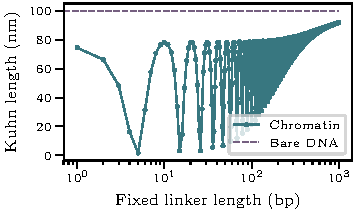
\includegraphics{./figures/fig2b_kuhn_length_homogenous_1to1000links_0unwraps.pdf}

%     }%
%     \subfloat[][]{\label{fig:homo-kuhn-zoom}
%         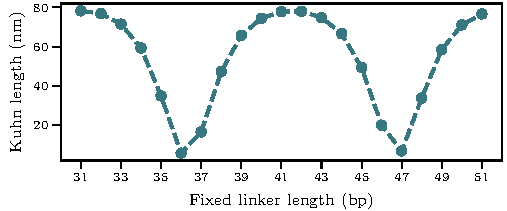
\includegraphics{./figures/fig2c_kuhn_length_in_nm_31to51links_0unwraps.pdf}
%     }%
%     \end{centering}
%     \caption{\protect\subref{fig:mc-example} Zero-temperature structure vs.
%     Monte Carlo simulation snapshot of nucleosome chain with \SI{38}{\basepair}
%     linkers.  \protect\subref{fig:homo-kuhn-all} The Kuhn lengths of homogenous
%     chains are \SI{10.5}{\basepair} periodic in linker length, with each linker
%     length representing a distinct, discretized helical WLC\@. In the limit of
%     long linkers, the Kuhn length eventually approaches that of bare DNA,
%     \SI{100}{\nano\metre}. \protect\subref{fig:homo-kuhn-zoom} Compact,
%     superhelical structures afford more flexibility than non-compact fibres,
%     which have higher Kuhn lengths. Thus, the overall structure of chromatin is
%     extremely sensitive to changes in the nucleosome repeat
%     length.}\label{fig:homo-kuhn}
% \end{figure*}

\section{\label{sec:results}Results}
%% introduce our strategy: zero-temperature to build intuition
We begin by comparing the Kuhn length of chains with various linker length
    distributions to their zero-temperature (i.e.\ minimum-energy) structure.
%% what is a kuhn length
Recall that the Kuhn length, $b$, is a universal measure of the long-length
    scale behavior of a polymer.
%%why do we care about the kuhn length?
For any polymer model, the mean end to end distance $\RR$ is linearly related to the
    underlying chain length, $L$, by $\RR = bL$ for large enough $L$.
For the wormlike chain, the Kuhn length is directly related to the elasticity of
    the chain via it's persistence length $b = 2l_p$.

\begin{figure}
    \mbox{\includegraphics{../../deepti/nuc_chain_tmp/plots/PRL/fig2a_r2_homogenous_vs_wlc-scaled.pdf}
    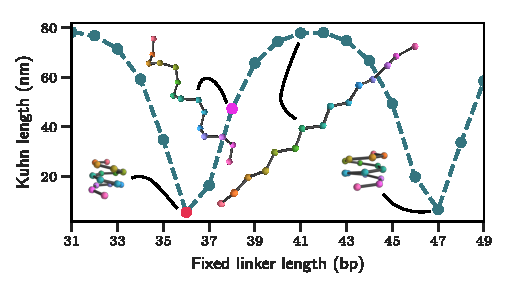
\includegraphics{../../deepti/nuc_chain_tmp/plots/PRL/fig2b_kuhn_length_in_nm_31to51links_0unwraps-with-renderings.pdf}}
    \caption{homogenous chain stuff.}\label{fig:homo-chain}
\end{figure}

%% homo-chain r2 example, compare to WLC, notice don't match
We compare $\sqrt{\RR}$ as a
function of cumulative chain length for a homogenous chain of
nucleosomes with \SI{36}{\basepair} linkers to that of the best-fit WLC without
kinks in Figure~\ref{fig:r2-homo-wlc}.
For a WLC, the initial slope in log-log space of $\sqrt{\RR}$ is one,
    corresponding to rigid rod behavior at short length scales.
Around it's persistence length, this slope transitions to $1/2$, corresponding
    to diffusive behavior at long length scales.
In contrast, the short length scale behavior of the homogenous kinked chain is more
    complex. Even when the linkers are effectively rigid rods, they trace
    out a non-linear path due to the rigid angles that connect them.
Thus, even though the WLC was chosen to match the Kuhn length of this
    homogenous chain, our full theory is required to describe the short length
    scale behavior. On the flip side, a WLC with a persistence length chosen to fit the short length-scale behavior of the nucleosome chain will fail to capture the large-scale behavior.

%%here's what determines the kuhn length: zero temperature picture
In order to extend this geometric intuition to longer length scales, we extract
the Kuhn lengths from the $\RR$ of fluctuating chains, and compare them to
    the corresponding  zero-temperature configurations, where the entire chain is
    composed of rigid rod linkers.
In Figure~\ref{fig:homo-kuhn-zoom},% In our model, the chain fluctuates thermally around this minimum energy
%     configuration by an amount determined by the persistence length of the
%     linkers ($l_p \approx \SI{50}{\nano\metre}$), and it is this fluctuating
%     chain that the Kuhn length is measuring.
we observe that the chains with more ``processive'' minimum energy structures
    are exactly those with larger Kuhn lengths.
%% what determines zero temperature pictures for homogenous chain
More precisely, every homogenous chain at zero temperature forms a
    %BRUNO: I think explicitly pointing out that it's a superhelix is actually
    %MORE confusing than not. esp sicne we already say "of nucleosomes"
    helix of nucleosomes (as a consequence of Chasles' theorem).
The rise per basepair of the helix is determined by the spherical angles
    $\theta$ and $\phi$ connecting adjacent linkers (Figure~\ref{fig:nuc-geo}).
The nucleosome structure fixes $\theta$, but $\phi$ depends linearly on the
    linker length, and is \SI{10.5}{\basepair} periodic due to DNA's helicity.
For realistic linker lengths, this periodicity largely determines the
\SI{10.5}{\basepair} periodic oscillations in the Kuhn
length, as seen in Figure~\ref{fig:homo-kuhn-zoom}.
Select values of $\phi$ lead to more compact zero-temperature structures with a
smaller rise/bp. By extension, the corresponding fluctuating structures have smaller Kuhn
lengths.

For arbitrarily long linker lengths, $\meanli\to\infty$, this relationship breaks
    down as thermal fluctuations begin to dominate the linker behavior (see
    Figure~\ref{fig:homo-kuhn-large}).
However, this breakdown is slow, since the kink density decreases as $1/\meanli$.

%% conclusion on sensitivity of Kuhn length to NRL for homo case,
Due to the dominance of geometrical effects for realistic linker lengths, the
Kuhn length is extremely  sensitive to the particular choice of linker length.
%% transition to heterogenous chains
Because of this sensitivity, we hypothesized that introducing modest amounts of
    heterogeneity in the linker length could significantly affect the geometric
    and physical organization of the chromatin chain.

\begin{figure}
    \centering
    \includegraphics{../../deepti/nuc_chain_tmp/plots/PRL/fig-3-kuhn_length_vs_window_size_41_sigma0to40-v4.pdf}
    \caption{Increasing sigma}
\end{figure}

%% what determines zero temperature picture for het chains
We apply our fluctuating theory to study the chains first considered
    in~\cite{woodcock1993}, where the linker lengths are drawn uniformly from a
    range $\mu \pm \sigma$.
As in the homogenous case, the processivity of the zero-temperature
    configuration qualitatively explains the Kuhn length of the fluctuating chain.
In Figure~\ref{fig:hetero-geom}, we see that as we increase $\sigma$, the
    zero-temperature configuration of the chain interpolates between a helix at
    $\sigma = 0$ and a random walk at larger $\sigma$.
This is because as we increase $\sigma$, the distribution of $\phi \in [0, 2\pi]$ connecting
    adjacent linkers quickly becomes approximately uniform.
A random walk where steps are taken with fixed $\theta$ and uniformly
    random $\phi$ is known as a freely-jointed chain.
Our zero-temperature structures are a generalization of this concept where step
    sizes and $\phi$ are correlated.

%% how do zero temp and fluct pictures compare?
Since the zero temperature structure becomes a random walk at long length
    scales, we use its diffusivity (i.e.\ its effective Kuhn length) as our
    measure of processivity.
Figure~\ref{fig:hetero-kuhn-unif} shows how the Kuhn lengths of the
zero-temperature and fluctuating structures qualitatively follow the same trend
as $\sigma$ increases.
%thoughts on cutting the next sentence? if we include it, think it needs more
%explanation. or we could just put this in the discussion.
%This stands in contrast to existing methods for combining the Kuhn lengths of
%    heterogenous polymer chains based on Rouse theory (Supplemental Figure XX).
Thus, we conclude that the geometric effects imposed by
    stochastic nucleosome spacing dominate the thermal fluctuations of the
    polymer when determining the structure of the chromatin chain.

%% universality and it's approached quickly
We also notice that the Kuhn length rapidly converges to
a constant value as $\sigma\to\infty$.
The convergence rate corresponds to how quickly $\phi$ becomes approximately
    uniform as $\sigma$ increases.
In order to highlight the transition from rigid helix to a random walk, a slowly
    converging case was chosen.
However, for many average linker lengths, the Kuhn length has essentially
    converged with as little as $\sigma = \SI{1}{\basepair}$ of variability in
    linker lengths (Supplemental Figure XX).

%% introduce maximum entropy limit
We can understand the structure to which our heterogenous chains converge by studying the
maximally entropic linker length distribution. The homogenous case ($\sigma=0$) is the
    minimum entropy arrangement of nucleosomes for a given $\meanli$. In
    contrast, in the maximum entropy arrangement, molecules bind uniformly to
    the lattice. For a sufficiently large lattice, the distances separating the
    molecules are well-approximated by exponential, i.i.d.\ random variables.
This is also exactly the distribution implied by  state-of-the-art models of nucleosome
    positioning ~\cite{beshnova2014}.

%%universality, justify exponential
We find that the Kuhn lengths for chains sampled from a
uniform linker length distribution rapidly converge to this
maximum entropy limit as $\sigma\to\infty$.  
The fact that the limiting value is distribution-free suggests that even if nucleosomes were  positioned more precisely than predicted by current models, exponentially distributed linker lengths would remain an excellent approximation, as long as $\phi$ remains approximately uniform.

\begin{figure}
    \centering
    \mbox{\includegraphics{../../deepti/nuc_chain_tmp/plots/PRL/fig4a_r2_exp_vs_wlc-scaled.pdf}
    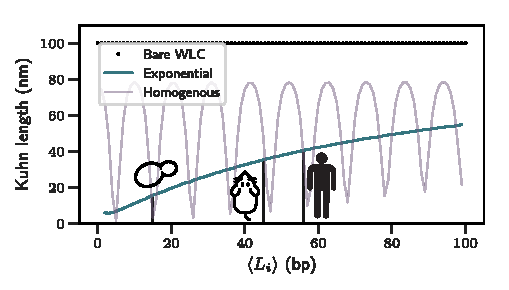
\includegraphics{../../deepti/nuc_chain_tmp/plots/PRL/fig4b_kuhn_exponential-with-images.pdf}}
    \caption{universal chain Kuhn length}\label{fig:exp-chain}
\end{figure}


%% R^2 of exponential chains, match WLC, that's also good, need only Kuhn length
Motivated by this fact, we compare the $\RR$ for various
    ``exponential'' chains  with a WLC with the same Kuhn length in Figure~\ref{fig:exp-r2}.
Unlike in the homogenous chain case, both the short and large size scales are
    well explained by a single effective WLC.\@
This means that in this universal limit of uniform $\phi$, coarse-graining
    chromatin's structure only requires  computing the Kuhn length of the
    exponential chain for the desired $\meanli$, which varies based on the cell
    type.

%% we compute kuhn length, not sensitive like in homo chain
In Figure~\ref{fig:hetero-kuhn}, we compute the Kuhn lengths of our exponential
    chain as a function of $\meanli$.
Because increasing linker lengths only scales the random walk, the Kuhn length
    lacks the \SI{10.5}{\basepair} periodicity of the homogenous chain.
This means that chromatin's large scale behavior is less sensitive to
    the nucleosome repeat length than previously predicted in the homogenous
    case.
A table of these Kuhn lengths is available in Supplemental Table XX, and we
    emphasize that an approximate knowledge of the NRL should be sufficient for
    the purposes of coarse-graining.

%% trans to looping
Next, we wondered how much rearranging the nucleosomes between two
    loci could affect the ability of chromatin loops to form.
Since our theory allows an analytical solution, we can probe this question
    systematically for the first time.
In Figure~\ref{fig:looping}, we compute the propensity of individual chromatin
    chains drawn from the maximum entropy distribution to form loops as a
    function of the loop size.

\begin{figure}
    \centering
    \includegraphics[width=0.95\linewidth,height=0.4\linewidth]{../../deepti/nuc_chain_tmp/plots/PRL/fig5_looping_hetero31to52bp_bold3curves.pdf}
    \caption{looping stuff.}
\end{figure}

%% general features
As expected, the typical model of chromatin as bare DNA systematically
    underestimates the looping propensity, because of the reduced Kuhn length of
    the chromatin chain.
%% slow nucleosome turnover
Strikingly, we observe that the difference between the most- and least-likely to
    loop loci spans six orders of magnitude.
As suggested by our previous results, this huge inter-chain variability is
    driven primarily by the different geometrical properties of individual
    chromatin chains (Supplemental Figure XX showing compact and straight homo chains
    looping).
These results imply that loop formation on time scales shorter than nucleosome
    turnover can be dramatically influenced by local changes to nucleosome
    positioning.

%%fast nucleosome turnover, implications for multiscale modeling
For time scales much longer than nucleosome turnover, our results mirror those
    in Figure~\ref{fig:hetero-kuhns}.
As can be seen in Figure~\ref{fig:looping}, the best fit wormlike chain is able
    to capture the probability of DNA contacts as a function of genomic separation.
We note that the kilobase-range peak of the average chain exactly corresponds to
    the characteristic length-scale of enhancer-promoter contacts.
At longer length scales, the looping probability approaches that of a Gaussian
    chain with the familiar $L^{-3/2}$ scaling.
%TODO continue

\section{\label{sec:discussion}Discussion}
%this feels redundant with the intro
%The dependence of chromatin's structure on the length of its linkers has been
%    widely discussed since at least the 70's~\cite{finch1976}.
%%ugh, phrase this better
%However, likely because of a lack of a unifying analytical theory, models
%    including heterogenously spaced nucleosomes have been comparably
%    rare~\cite{woodcock1993,collepardo-guevara2014}.

We present a simplified model of the chromatin fiber that retains only the most
    basic geometrical and physical properties of a chain of nucleosomes
    connected by bare linker DNA.\@
By taking a fully analytical approach, we are able to outline the effects of
    linker length and its heterogeneity on the structure of the chromatin fiber.

Our model excludes various important facets of chromatin's structure.
Most strikingly, we ignore the steric interactions between nucleosomes that is
    well known~\cite{widom1992} to constrain the space of possible linker
    lengths.
In addition, our model ignores the finite size of the nucleosome, treating it as
    a point-like kink in the DNA backbone.

While these choices constrain the ability of our model to make predictions that
    can be tested \textit{in vivo}, our bottom-up approach allows us to
    formalize both new and existing intuition for how linker length affects the
    structure of the chromatin fiber in a unified framework.
% We hope that our framework will facilitate future analytical work that takes
%     these details, and many more, into account.
We expect that our central conclusions---that nucleosomes can modulate
    chromatin's elasticity and facilitate or prevent looping between distal loci
    through their positioning---will only gain nuance as these details are added
    to future analytical works.

    %TODO add this sentence into the flow somewhere around here
    For example, DNA is known to partially unwrap from the nucleosome core dynamically \textit{in
% I have tons of citations for these two statements in zotero, just have to
% separate them from each other tediously to make two lists
    vivo}, whether spontaneously (called nucleosome breathing~\cite{TODO}), due to
    force on the DNA~\cite{TODO}, or through active
    remodelling~\cite{dion2007,kulaeva2007,senavirathne2017}. Stochastic
    unwrapping will cause the angle $\theta \in [0, \pi]$ between adjacent nucleosomes to
    also become approximate uniform. In this limit, the nucleosome chain is an
    ideal chain with bond-length-phi correlation and fluctuating linkers. 
    
    In future work, we plan to explicitly incorporate the energetics of nucleosome unwrapping
    and repositioning to predict how these quantities affect the dynamic
    organization of chromatin. In particular, this will allow us to more
    precisely understand how chromatin remodelers affect chromatin loop
    formation.

While the quantitative values may yet change from these additions, we suspect that our estimate of chromatin's Kuhn length and looping probabilities will already provide
    guidance to future coarse-grained models of chromatin.
We show that the common practice~\cite{macphersonInPress,nuebler2018}
    of using a Kuhn length of \SI{100}{\nano\metre}, simply because that is the
    Kuhn length of bare DNA, will likely lead to at least a four-fold
    overestimation of the polymer's stiffness. %is this verified?
In large-scale models of chromatin organization, this could mean the difference
    between heterochromatin and euchromatin segregation recapitulating
    \textit{in vivo} observations, and the chromosomes instead being uniformly
    distributed throughout the nucleus.

It is interesting to note that the helical wormlike chain has been employed
    in the past to explain the looping statistics of bare DNA~\cite{shimada1984,
    liu2011a}.
Along with the so-called ``kinked'' wormlike chain model~\cite{wiggins2005,
    popov2005}---where kinks are flexible, and represent melted base
    pairs---these models were created to explain the propensity for small DNA
    loops \textit{in vivo}.
Our model highlights that even without models of DNA more detailed than the WLC,
    the looping probabilites for short segments of DNA can be increased by
    orders of magnitude simply by the specific or non-specific binding of any
    protein that promotes a kink in the DNA.\@

Finally, while our model has been designed specifically to address chromatin
    structure, we suspect that the intuition gained here will also apply more
    broadly to block copolymers in solution.
Typical block copolymers have a dihedral ``kink'' at the junctions between
    blocks, and our framework could easily be applied to any particular
    copolymer of interest to relate the elasticity and circularization
    propensity of the polymer to the the block size, analagously to linker
    length.
Since in this analogy, there is no way for the kinks to reposition themselves,
    our results apply in the limit of slow nucleosome turnover.
Our results suggest that cyclizability of copolymers could be increased by
    encouraging heterogenous block sizes.
In addition, our results imply that the observed persistence lengths of block
    copolymer could vary drastically from that predicted from the Kuhn lengths
    of their constituent blocks, depending on the block size.

%TODO: not sure if this needs to go in discussion for this paper
propose that we should use this new model to look at supercoiling effects
of nucleosome positions as proposed in~\cite{grigoryev1981} (some paradoxes
about this~\cite{prunell1998} were later solved in~\cite{nikitina2017}

%TODO: added this
propose more comprehensive understading of ability of chromatin
remodellers to affect structure using our model, instead of
e.g.~\cite{muller2014} where they only ``move'' one nucleosome
specifically, propose to add energetics for unwrapping explicity, remodeling
expclicitly.

%TODO: not sure if we need this
make sure we mention that although increasingly high-fidelity measurements
of nucelsoome position continue to suggest that linker lengths are
preferentially quantized, this does not exclude them not being perfectly
quantized. (probalby in introducetion to section on "uniformly dist" linker
lengths

%TODO: added this
discuss how our universal chain is like the hindered rotating chain, and
how unwrapping would make that like an ideal cahin, and in both cases the
difference with our model is that there's 1) bond length-phi correlation 2)
thermal fluctuations of the linkers


% \subsection{\label{sec:homo-chain}Homogenous Chains}

% We first revisit the illustrative case of a homogenous chromatin chain, where
%     there is a constant linker length separating adjacent nucleosomes.
% In the simplifying limit of zero temperature, the linkers are rigid rods, and
%     our model is purely geometrical.
% The geometrical model with constant linker lengths traces out a helix whose
%     pitch is determined solely by the spherical angles $\theta$ and $\phi$
%     connecting adjacent linkers.
% The angle $\theta$ is fixed by the structure of the nucleosome
%     (Figure~\ref{fig:entry-exit}), but the angle $\phi$ between linkers depends
%     on the linker length (Figure~\ref{fig:linker-effect}).

% In Figure~\ref{fig:homo-kuhn-zoom}, the Kuhn length of the
%     fluctuating homogenous chain is compared to the geometric model for
%     typical linker lengths.
% Since these linkers are much shorter than the \SI{150}{\basepair} persistence
%     length of bare DNA, the linkers are approximately rigid rods, and the Kuhn
%     length corresponds directly to the shape of the geometric model.

% In the short-length limit, the Kuhn length is approximately \SI{10.5}{\basepair}
%     periodic.
% This reflects the \SI{10.5}{\basepair} helical periodicity of dsDNA.\@
% In the limit as the linker length increases, the Kuhn length approaches that of
%     bare DNA.\@
% However, since the kink density is proportional to the inverse of the linker
%     length, this happens slowly (like $1/L_i$), and for realistic linker
%     lengths, only $\phi$ matters (Figure~\ref{fig:homo-kuhn-zoom}).

% %TODO NEW FIGURE 1a. It will simply show one $\RR$ curve and the best fit WLC
%     %near the start of the curve and the best fit gaussian chain nithe long
%     %chain limit.
% For a regular wormlike chain, the Kuhn length $b = 2 l_p$.
% However, Chasles' theorem makes homogenous chains of nucleosomes ``helical''
%     wormlike chains~\cite{yamakawa2016}.

% However, for the helical wormlike chain, amount of DNA contained per unit of
%     rise along the nucleosomal helix, as shown in
%     Figure~\ref{fig:homo-kuhn-zoom}.
% %TODO: add the example structures back in

% Perhaps most notably, the variability between the stiffest and most flexible
%     chromatin chains spans over an order of magnitude in Kuhn lengths.
% %TODO: color the inaccessible ones
% While some of the most compact configurations will sterically inaccesible, this
%     demonstrates the drastic effect that nucleosome binding can have on DNA's
%     elasticity.

% At short length scales, the $\RR$ behaves like a wormlike chain with reduced
%     persistence length, due to the linkers being forced to traverse a helix.
% At long length scales, the chain predictably asymptotes to a Gaussian
%     chain, again with reduced Kuhn length compared to the underlying linkers.
% It is noteworthy that the best fit persistence length at short scales and the
%     best fit Kuhn length at long scales are quite different (Supplemental Figure
%     XX).
% Thus, our full theory is required even for calculations involving this
%     simplified, homogenous chromatin chain.


% \subsection{\label{sec:hetero-kuhn}Heterogenous Nucleosome
% \texorpdfstring{$\RR$}{<R2>}}

% We now consider the more relevant scenario, when the nucleosomes are randomly
%     spaced along the DNA backbone.
% %TODO say what we do first, then why we do it
% While certain DNA sequences have higher affinities for
%     nucleosomes~\cite{something widom}, in practice the most striking features
%     of nucleosome positioning data are nucleosome phasing near promoters, CTCF
%     sites, and other sites that sterically inhibit nucleosome
%     binding~\cite{widom1992}.
% These features are predicted to occur by the simplest model of nucleosome
%     positioning, one where nucleosomes are positioned uniformly along the DNA
%     backbone, and simply sterically excluded from certain sites.
% In terms of linker lengths, this model corresponds approximately to the case
%     where linker lengths are independent and exponentially distributed about
%     their mean.
% Thus, while the exact statistics of \textit{in vivo} linker lengths remain to be
%     determined, we use the case of independent, exponentially distributed
%     linkers as a reference point to show the effect of linker heterogeneity on
%     the statistical mechanics of the chromatin fiber.

% In analogy to the case of homogenous chains, we find that the zero temperature
%     structure provides good intuition for the behavior of the chromatin chain
%     when thermal fluctuations are added.
% At zero temperature, a chain with random linker lengths is going to have a
%     structure determined purely by the interactions between the nucleosome geometry
%     and the DNA's intrinsic twist.
% In our model, the angle $\theta$ in Figure~\ref{fig:entry-exit} is fixed by the
%     nucleosome geometry, but the angle $\phi$ in Figure~\ref{fig:linker-effect}
%     is determined by linker length.
% As the heterogeneity in linker length increases, this means that the
%     zero temperature heterogenous chain will interpolate between a rigid helix
%     (in the case of zero linker length variability) and a modified freely
%     rotating chain (in the case when linker variability is high enough to make
%     the distribution of $\phi$ approximately uniform over $[0, 2\pi]$).

% %TODO reincorporate somewhere around here
% %DEEPTI:it's not just random right? hasn't shlick done the Oct4 gene with
%    %nucleosome positioning data?
% %BRUNO:I assume you mean Bascom 2017? yeah but I mean they still use random linker
%    % lengths...just like we do
% Simulations of particular chromatin chains with random linker lengths have
%     suggested that heterogeneity in nucleosome spacing leads to largely
%     disordered chromatin architecture~\cite{woodcock1993,
%     collepardo-guevara2014, bascom2017a} reminiscent of modern electron
%     microscopy images~\cite{ou2017}.
% %DEEPTI:maybe it's just me, but why cite the older paper if more recent models do
% %include fluctuations?
% %BRUNO: if I have two citations, I always put the
% %"foundational" one and the "most recent" one. plus it's two different
% %groups, you kinda want one citation per group to independently do a thing.
% %alos, why not have all three citations? personally I feel like...just cite
% %everyone, why not? especially since there's so few peopel to cite

% % \begin{figure}[t]
% %     \centering
% %     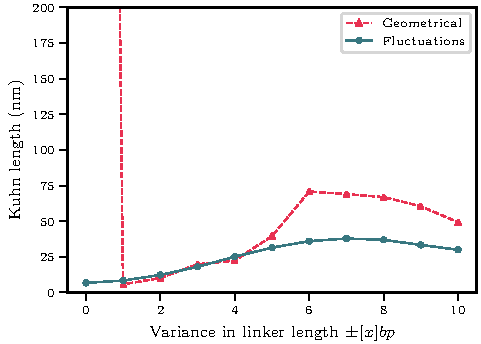
\includegraphics{./figures/fig4_kuhn_length_vs_window_size_mu47bp.pdf}
% %     \caption{Kuhn lengths for heterogenous chains as a function of
% %      the amount of variance in the uniformly distributed linker lengths with a mean
% %      of \SI{47}{\basepair}. Adding merely \SI{1}{\basepair} of variability causes the
% %      zero-temperature configuration (red triangles) to resemble a random walk with ``Kuhn
% %      length'' (i.e.\ diffusivity) drastically lower than that of bare DNA
% %      (\SI{100}{\basepair}), explaining the heterogenous chain's increased
% %     flexibility.}\label{fig:box-kuhns}
% % \end{figure}


% % \begin{figure}[t]
% %     \centering
% %     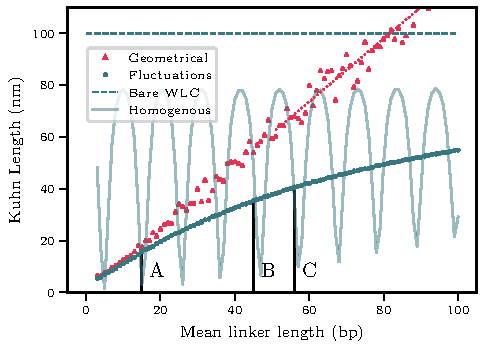
\includegraphics{./figures/fig3_kuhn_exponential.pdf}
% %     \caption{We compare the kuhn lengths of realistic chromatin fibers
% %     against those of the corresponding zero-temperature configurations (red
% %     triangles) and bare DNA (dashed line). Geometrical kinks and fluctuations
% %     combine to drastically increase the elasticity of chromatin. With exponentially
% %     distributed linker lengths, the kuhn length smoothly increases as a function
% %     of the mean linker length, and dampens the chaotic oscillations in the kuhn
% %     lenghts of homogenous chains. Mean linker
% %     lengths in \textit{S.  cerivisiae}[Chereji] (A), mice embryonic stem cells
% %     [Voong] (B), and human T cells  [Valouev] (C)  are marked.}\label{fig:exp-kuhns}
% % \end{figure}

% As expected, for short linker lengths, $<\SI{20}{\basepair}$, the
%     zero-temperature, ``geometric'' model predicts the Kuhn length of the chain
%     extremely well (Figure~\ref{fig:exp-kuhns}).
% As the average linker length
%     increases, the geometric picture becomes increasingly processive since each
%     linker is still a rigid rod.
% On the other hand, the fluctuating chain's Kuhn length stays markedly below the
%     \SI{100}{\nano\metre} Kuhn length of the underlying DNA backbone.
% While the Kuhn length approaches \SI{100}{\nano\metre} as the linker length
%     increases to infinity, this approach is power-law slow (difference shrinks
%     as inverse of the linker lengths, see Supplemental Figure XX).
% In fact, for realistic linker lengths, the effect is at least a factor of 2.

% While exponentially-distributed linker lengths seem like the most natural
%     baseline to take, it is equally natural to ask how much variability in the
%     nucleosome spacing is needed to create this effect.
% While the answer varies depending on the mean linker length to some degree (see
%     Supplemental Figure XX for more examples), we show in
%     Figure~\ref{fig:box-kuhns} that as little as one base pair of variability
% %TODO this statement is almost certainly too strong
%     can lead to the chromatin fiber's structure being governed by the
%     nucleosome's geometrical properties.

% \subsection{\label{sec:looping}Effects of Nucleosome Spacing on Chromatin
% Looping}

% Chromatin looping is central to biological processes from transcriptional
%     control (e.g.\ via promoter-enhancer search) to DNA damage repair (e.g.\ via
%     homologous recombination).
% In Figure~\ref{fig:looping}, we evaluate our Green's function at $\vec{R} = 0$
%     for an ensemble of chains with linker lengths drawn from an exponential
%     distribution with mean \SI{54}{\basepair} (using a uniform distribution
%     yields similar results, see Supplemental Figure XX).
% This quantity quantifies the propensity for two loci on the same chromosome to
%     come into contact with each other as a function of their genomic separation.
% As expected, the large length scale behavior matches the Gaussian chain scaling
%     of $L^{-3/2}$, with the Kuhn length predicted by our earlier analysis.

% In comparison to bare DNA, we find that the looping propensity increases
%     drastically along the entire chain, as expected due to intra-superhelical
%     contacts induced by the nucleosomes' geometry, as well as due to the
%     increased elasticity predicted by the model.
% More striking than the increase in the looping propensity is the nearly four
%     orders of magnitude over which specific rearrangement of nucleosomes can
%     modulate the ability of two loci to loop together.
% Even at long length scales, where the chain is approximately Gaussian, it is
%     possible to increase or decrease the rate of looping by over an order of
%     magnitude.
% This has profound implications for the ability of chromatin remodelers to act in
%     way that can bring together or keep apart related chromosomal loci based on
%     the epigenetic environment.

% % \begin{figure}[t]
% %     \centering
% %     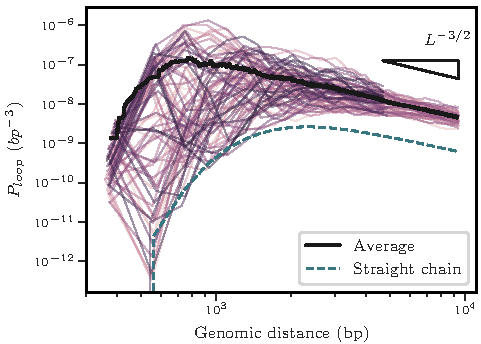
\includegraphics{./figures/fig5_looping_hetero31to52bp.pdf}
% %     %\includegraphics[width=0.35\linewidth]{./figures/fig-5b-looping-features.png}
% %     \caption{Each purple line designates an individual chain configuration
% %     with uniformly random linker lengths between 31 and \SI{51}{\basepair}, with
% %     the black line representing the average over individual chains. Thus, modulating nucleosome positions can allow the cell to change
% %     the probability of inter-nucleosomal contacts by up to 6 orders of
% %     magnitude. The peak in the average curve occurs at around a kilobase, the
% %     length scale of enhancer-promoter contacts. Although the average,
% %     heterogenous chain tends towards a Gaussian chain with a shorter
% %     effective Kuhn length, individual configurations retain memory of rigid kinks
% %     at intermediate length scales, as indicated by residual peaks in the looping
% %     probability.}\label{fig:looping}
% % \end{figure}

% Like the Kuhn length, our looping function is largely determined by the
%     geometrical properties of the underlying zero-temperature chain.
% In Figure~\ref{fig:looping}, two examples of homogenous chains with extremely
%     compact or extremely linear geometries are provided to show this.
% This suggests that \textit{in vivo}, looping propensity might be largely
%     determined by geometrical considerations, at least much more than it is
%     determined by the thermal fluctuations in the chromatin fiber.

% We notice that the size scale at which this is most true, around
%     \SI{1}{\kilo\basepair}, is concommitant with the sizes of loops that must
%     %TODO honestly i'm out of brain juice to word this carefully
%     often form to construct the transcription initiation complex.
% This suggests that the aforementioned phasing of nucleosomes near promoters
%     might play a causal role in transcription initiation or repression, and not
%     just be a side effect of steric exclusion.

% Finally, we note that even though the polymer rapidly approaches the Gaussian
%     scaling of $L^\alpha$ where $\alpha \approx -3/2$, the chain is slightly
%     non-Gaussian (i.e.\ $\alpha \gtrapprox -3/2$) for size scales even
%     approaching that of a full chromosome.
% This means that even large-scale, coarse-grained models of chromatin are likely
%     to fall short if they rely on Rouse (or WLC) looping probabilities.
% This is especially relevant to modeling epigenetic spreading, which requires
%     understanding the propensity nucleosomes at various distances have to loop with
%     each other.

% \section{PRL Guidelines}

% Must be submitted to a section, closest fit seems to be
% L8--81: Biological and Medical Physics

% Other options:
% L0--06: Statistical Physics and Thermodynamics
% L3--30: Dynamics and Structure of Atoms and Molecules
% L6--60: Chemical Physics
% but espeically these two:
% L8--78: Liquid Crystals and Polymers


% 3750 words

% Include:

% Any text in the body of the article;
% Any text in a figure caption or table caption;
% Any text in a footnote or an endnote

% Exclude:

% Title;
% Author and affiliation listing;
% Abstract;
% Receipt date, published date, and other publication history;
% PACS or Keywords and DOI;\@
% References;
% Author byline footnotes;
% Acknowledgments

% Estimating the word equivalent for figures can be simplified by using the aspect
% ratio (width / height) of the figure. The estimates would be ((150 / aspect
% ratio) + 20 words) for single-column figures, and ((300 / (0.5 * aspect ratio))
% + 40 words) for double column figures.

% The word equivalent for displayed math is 16 words per row for single-column
% equations. Two-column equations count as 32 words per row.

% % \section{\label{sec:level1}First-level heading}

% % This sample document demonstrates proper use of REV\TeX~4.1 (and
% % \LaTeXe) in mansucripts prepared for submission to APS
% % journals. Further information can be found in the REV\TeX~4.1
% % documentation included in the distribution or available at
% % \url{http://authors.aps.org/revtex4/}.

% % When commands are referred to in this example file, they are always
% % shown with their required arguments, using normal \TeX{} format. In
% % this format, \verb+#1+, \verb+#2+, etc. stand for required
% % author-supplied arguments to commands. For example, in
% % \verb+\section{#1}+ the \verb+#1+ stands for the title text of the
% % author's section heading, and in \verb+\title{#1}+ the \verb+#1+
% % stands for the title text of the paper.

% % Line breaks in section headings at all levels can be introduced using
% % \textbackslash\textbackslash. A blank input line tells \TeX\ that the
% % paragraph has ended. Note that top-level section headings are
% % automatically uppercased. If a specific letter or word should appear in
% % lowercase instead, you must escape it using \verb+\lowercase{#1}+ as
% % in the word ``via'' above.

% % \subsection{\label{sec:level2}Second-level heading: Formatting}

% % This file may be formatted in either the \texttt{preprint} or
% % \texttt{reprint} style. \texttt{reprint} format mimics final journal output.
% % Either format may be used for submission purposes. \texttt{letter} sized paper should
% % be used when submitting to APS journals.

% % \subsubsection{Wide text (A level-3 head)}
% % The \texttt{widetext} environment will make the text the width of the
% % full page, as on page~\pageref{eq:wideeq}. (Note the use the
% % \verb+\pageref{#1}+ command to refer to the page number.)
% % \paragraph{Note (Fourth-level head is run in)}
% % The width-changing commands only take effect in two-column formatting.
% % There is no effect if text is in a single column.

% % \subsection{\label{sec:citeref}Citations and References}
% % A citation in text uses the command \verb+\cite{#1}+ or
% % \verb+\onlinecite{#1}+ and refers to an entry in the bibliography.
% % An entry in the bibliography is a reference to another document.

% % \subsubsection{Citations}
% % Because REV\TeX\ uses the \verb+natbib+ package of Patrick Daly,
% % the entire repertoire of commands in that package are available for your document;
% % see the \verb+natbib+ documentation for further details. Please note that
% % REV\TeX\ requires version 8.31a or later of \verb+natbib+.

% % \paragraph{Syntax}
% % The argument of \verb+\cite+ may be a single \emph{key},
% % or may consist of a comma-separated list of keys.
% % The citation \emph{key} may contain
% % letters, numbers, the dash (-) character, or the period (.) character.
% % New with natbib 8.3 is an extension to the syntax that allows for
% % a star (*) form and two optional arguments on the citation key itself.
% % The syntax of the \verb+\cite+ command is thus (informally stated)
% % \begin{quotation}\flushleft\leftskip1em
% % \verb+\cite+ \verb+{+ \emph{key} \verb+}+, or\\
% % \verb+\cite+ \verb+{+ \emph{optarg+key} \verb+}+, or\\
% % \verb+\cite+ \verb+{+ \emph{optarg+key} \verb+,+ \emph{optarg+key}\ldots \verb+}+,
% % \end{quotation}\noindent
% % where \emph{optarg+key} signifies
% % \begin{quotation}\flushleft\leftskip1em
% % \emph{key}, or\\
% % \texttt{*}\emph{key}, or\\
% % \texttt{[}\emph{pre}\texttt{]}\emph{key}, or\\
% % \texttt{[}\emph{pre}\texttt{]}\texttt{[}\emph{post}\texttt{]}\emph{key}, or even\\
% % \texttt{*}\texttt{[}\emph{pre}\texttt{]}\texttt{[}\emph{post}\texttt{]}\emph{key}.
% % \end{quotation}\noindent
% % where \emph{pre} and \emph{post} is whatever text you wish to place
% % at the beginning and end, respectively, of the bibliographic reference
% % (see Ref.~[\onlinecite{witten2001}] and the two under Ref.~[\onlinecite{feyn54}]).
% % (Keep in mind that no automatic space or punctuation is applied.)
% % It is highly recommended that you put the entire \emph{pre} or \emph{post} portion
% % within its own set of braces, for example:
% % \verb+\cite+ \verb+{+ \texttt{[} \verb+{+\emph{text}\verb+}+\texttt{]}\emph{key}\verb+}+.
% % The extra set of braces will keep \LaTeX\ out of trouble if your \emph{text} contains the comma (,) character.

% % The star (*) modifier to the \emph{key} signifies that the reference is to be
% % merged with the previous reference into a single bibliographic entry,
% % a common idiom in APS and AIP articles (see below, Ref.~[\onlinecite{epr}]).
% % When references are merged in this way, they are separated by a semicolon instead of
% % the period (full stop) that would otherwise appear.

% % \paragraph{Eliding repeated information}
% % When a reference is merged, some of its fields may be elided: for example,
% % when the author matches that of the previous reference, it is omitted.
% % If both author and journal match, both are omitted.
% % If the journal matches, but the author does not, the journal is replaced by \emph{ibid.},
% % as exemplified by Ref.~[\onlinecite{epr}].
% % These rules embody common editorial practice in APS and AIP journals and will only
% % be in effect if the markup features of the APS and AIP Bib\TeX\ styles is employed.

% % \paragraph{The options of the cite command itself}
% % Please note that optional arguments to the \emph{key} change the reference in the bibliography,
% % not the citation in the body of the document.
% % For the latter, use the optional arguments of the \verb+\cite+ command itself:
% % \verb+\cite+ \texttt{*}\allowbreak
% % \texttt{[}\emph{pre-cite}\texttt{]}\allowbreak
% % \texttt{[}\emph{post-cite}\texttt{]}\allowbreak
% % \verb+{+\emph{key-list}\verb+}+.

\bibliography{chromatin}

\end{document}
